\renewcommand\thetable{\arabic{chapter}-\arabic{table}}
%\renewcommand\thefigure{\arabic{chapter}-\arabic{figure}} 
\chapter{結論與討論}
\label{cha:conclusions}


\section{結論}

Conclusion


\section{未來展望} 



資料探勘可分為四種知識型態,包括了迴歸、分類、分群、關聯四種,本研究初期依據此四種型態分析設計了數個不同面向的探勘目標,其中迴歸分析中,主要的知識為重要屬性的關係模型,例如本研究中的耐震能力、補強經費與校舍基本設計參數間之關係模型即為此一類之資料探勘。而分類分析中,



,而目前主要的發展都在於迴歸和分類兩種形式的知識,因此本研究未來發展的其中一個方向就是繼續擴展探勘的知識種類,包括了分群形式和關聯形式的知識,都還有許多可能性。

\begin{figure}[hbtp]
  \begin{center}
    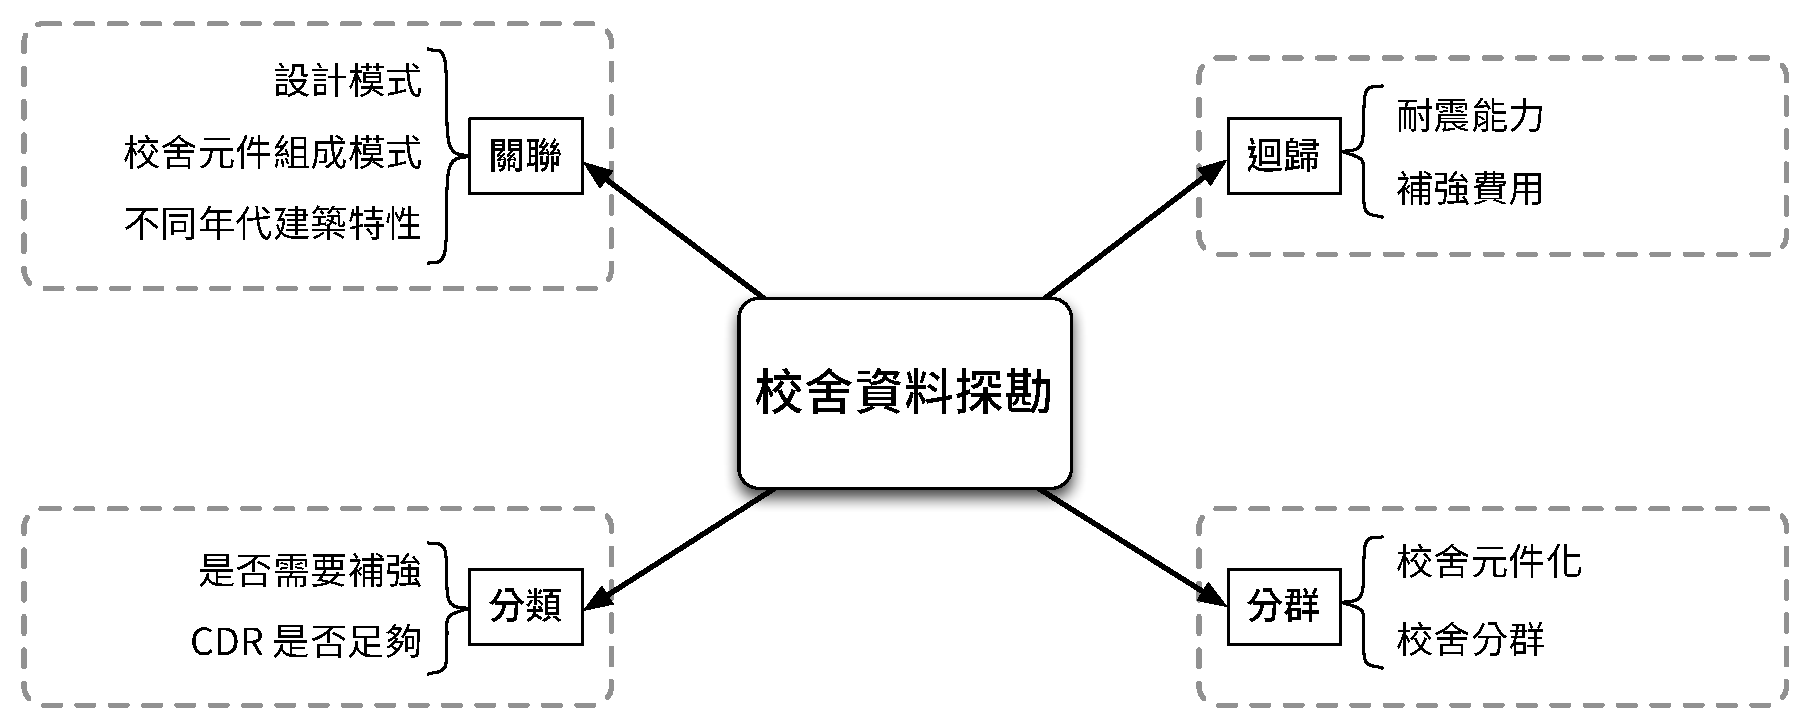
\includegraphics[width=1.0\textwidth]{figures/big-picture.pdf}
    \caption{知識挖掘規劃} 
    \label{fig:bigpicture}
  \end{center}
\end{figure}

另外一個發展方向,則是在 CRISP-DM 流程當中的最後一個步驟,將探勘得到的知識實際回饋到學校校舍及相關設備補強整建計畫上,由於目前探勘得到的知識都還是以數學模型的形式存在,非專業人士難以應用,因此如果可以將這些數學模型轉化成決策支援系統,則可以讓主管機關能夠簡單的得到這些模型的輔助,在校舍長期持續的耐震能力監控上,能夠發揮探勘所得知識的效力。


